\documentclass[parskip]{scrartcl}
\usepackage{geometry}
\usepackage{tikz}
\usetikzlibrary{3d,calc}

\begin{document}

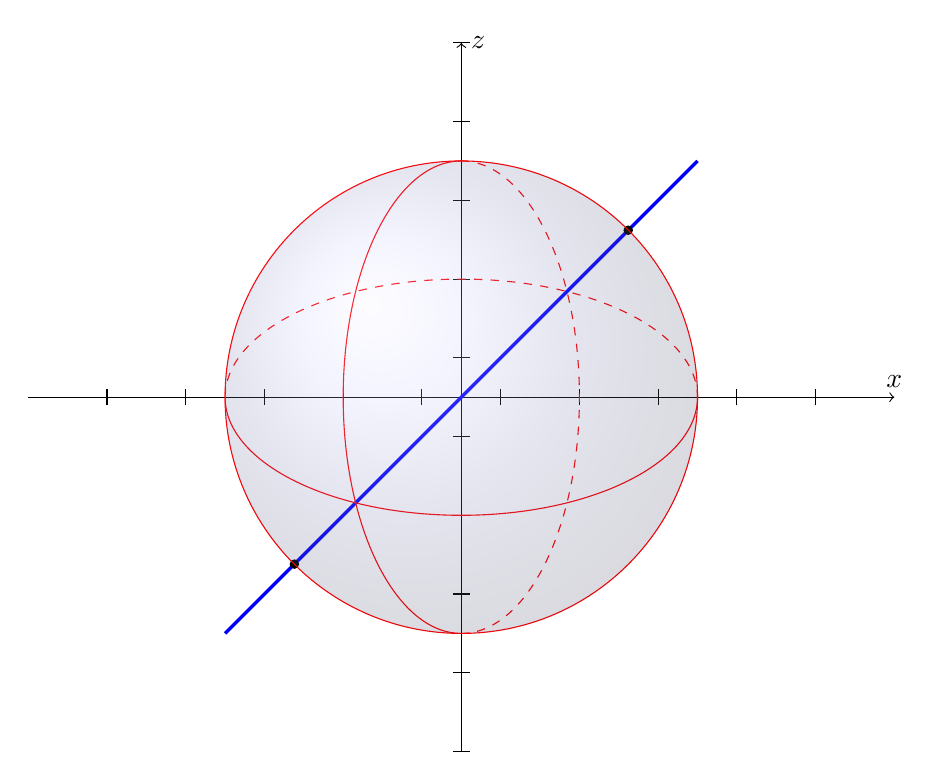
\begin{tikzpicture}

    % The axes
    \draw[->] (xyz cs:x=-5.5) -- (xyz cs:x=5.5) node[above] {$x$};
    \draw[->] (xyz cs:y=-4.5) -- (xyz cs:y=4.5) node[right] {$z$};
    % \draw[->] (xyz cs:z=-7.5) -- (xyz cs:z=7.5) node[above] {$y$};

    \foreach \coo in {-4.5,-3.5,...,4.5}
    {
        \draw (\coo, -3pt) -- (\coo,3pt);
        \draw (-3pt,\coo) -- (3pt,\coo);
        % \draw (xyz cs:y=-0.15pt,z=\coo) -- (xyz cs:y=0.15pt,z=\coo);
    }

    \draw[blue, very thick] (-3,-3) -- (3,3);
    \filldraw (2.12,2.12) circle[radius=1.5pt];
    \filldraw (-2.12,-2.12) circle[radius=1.5pt];

    \draw[red] (-3,0) arc (180:360:3cm and 1.5cm);
    \draw[red,dashed] (-3,0) arc (180:0:3cm and 1.5cm);
    \draw[red] (0,3) arc (90:270:1.5cm and 3cm);
    \draw[red,dashed] (0,3) arc (90:-90:1.5cm and 3cm);
    \draw[red] (0,0) circle (3cm);
    \shade[ball color=blue!30!white,opacity=0.20] (0,0) circle (3cm);
\end{tikzpicture}

\end{document}
